\documentclass[10.5pt]{article}

\usepackage{amsmath,amssymb,amsthm}
\usepackage{listings}
\usepackage{graphicx}
\usepackage[shortlabels]{enumitem}
\usepackage{tikz}
\usepackage[margin=1in]{geometry}
\usepackage{fancyhdr}
\usepackage{epsfig} %% for loading postscript figures
\usepackage{amsmath}
\usepackage{float}
\usepackage{amssymb}
\usepackage{caption}
\usepackage{subfigure}
\usepackage{graphics}
\usepackage{titlesec}
\usepackage{mathrsfs}
\usepackage{amsfonts}
\usepackage{indentfirst}
\usepackage{color}
\usepackage{algorithm}
\usepackage{algorithmicx}
\usepackage{algpseudocode}
\renewcommand{\baselinestretch}{1.2}%Adjust Line Spacing
%\geometry{left=2.0cm,right=2.0cm,top=2.0cm,bottom=2.0cm}% Adjust Margins of the File
\usepackage{tikz-qtree}
\usetikzlibrary{graphs}
\usetikzlibrary{shapes.multipart, matrix, backgrounds}
\tikzset{every tree node/.style={minimum width=2em,draw,circle},
	blank/.style={draw=none},
	edge from parent/.style=
	{draw,edge from parent path={(\tikzparentnode) -- (\tikzchildnode)}},
	level distance=1.2cm}
\setlength{\parindent}{0pt}
%\setlength{\parskip}{5pt plus 1pt}
\setlength{\headheight}{13.6pt}
\newcommand\question[2]{\vspace{.25in}\hrule\textbf{#1: #2}\vspace{.5em}\hrule\vspace{.10in}}
\renewcommand\part[1]{\vspace{.10in}\textbf{(#1)}}
%\newcommand\algorithm{\vspace{.10in}\textbf{Algorithm: }}
\newcommand\correctness{\vspace{.10in}\textbf{Correctness: }}
\newcommand\runtime{\vspace{.10in}\textbf{Running time: }}
\pagestyle{fancyplain}
% Create horizontal rule command with an argument of height
\newcommand{\horrule}[1]{\rule{\linewidth}{#1}}



% Set the title here
\title{
	\normalfont \normalsize
	\textsc{ShanghaiTech University} \\ [25pt]
	\horrule{0.5pt} \\[0.4cm] % Thin top horizontal rule
	\huge CS101 Algorithms and Data Structures\\ % The assignment title
	\LARGE Fall 2021\\
	\LARGE Homework 4\\
	\horrule{2pt} \\[0.5cm] % Thick bottom horizontal rule
}
% wrong usage of \author, never mind
\author{}
\date{Due date: 23:59, October 24, 2021}

% set the header and footer
\pagestyle{fancy}
\lhead{CS101 Algorithms and Data Structures}
\chead{Homework 4}
\rhead{Due date: 23:59, October 24, 2021}
\cfoot{\thepage}
\renewcommand{\headrulewidth}{0.4pt}
\newtheorem{Q}{Question}
% special settings for the first page
\fancypagestyle{firstpage}
{
	\renewcommand{\headrulewidth}{0pt}
	\fancyhf{}
	\fancyfoot[C]{\thepage}
}

% Add the support for auto numbering
% use \problem{title} or \problem[number]{title} to add a new problem
% also \subproblem is supported, just use it like \subsection
\newcounter{ProblemCounter}
\newcounter{oldvalue}
\newcommand{\problem}[2][-1]{
	\setcounter{oldvalue}{\value{secnumdepth}}
	\setcounter{secnumdepth}{0}
	\ifnum#1>-1
	\setcounter{ProblemCounter}{0}
	\else
	\stepcounter{ProblemCounter}
	\fi
	\section{Problem \arabic{ProblemCounter}: #2}
	\setcounter{secnumdepth}{\value{oldvalue}}
}
\newcommand{\subproblem}[1]{
	\setcounter{oldvalue}{\value{section}}
	\setcounter{section}{\value{ProblemCounter}}
	\subsection{#1}
	\setcounter{section}{\value{oldvalue}}
}

% \setmonofont{Consolas}
\definecolor{blve}{rgb}{0.3372549 , 0.61176471, 0.83921569}
\definecolor{gr33n}{rgb}{0.29019608, 0.7372549 , 0.64705882}
\makeatletter
\lst@InstallKeywords k{class}{classstyle}\slshape{classstyle}{}ld
\makeatother
\lstset{language=C++,
	basicstyle=\ttfamily,
	keywordstyle=\color{blve}\ttfamily,
	stringstyle=\color{red}\ttfamily,
	commentstyle=\color{magenta}\ttfamily,
	morecomment=[l][\color{magenta}]{\#},
	classstyle = \bfseries\color{gr33n}, 
	tabsize=4
}
\lstset{basicstyle=\ttfamily}
\begin{document}
	
	\maketitle
	\thispagestyle{firstpage}
	%\newpage
	\vspace{3ex}
	
	\begin{enumerate}
		\item Please write your solutions in English. 
		
		\item Submit your solutions to gradescope.com.  
		
		\item Set your FULL NAME to your Chinese name and your STUDENT ID correctly in Account Settings. 
		
		\item If you want to submit a handwritten version, scan it clearly. Camscanner is recommended. 
		
		\item When submitting, match your solutions to the according problem numbers correctly. 
		
		\item No late submission will be accepted.
		
		\item Violations to any of the above may result in zero grade. 
		
		\item Problem 0 gives you a template on how to organize your answer, so please read it carefully.
	\end{enumerate}
	\newpage

\problem[0]{Notes and Example}
\textbf{Notes}
\begin{enumerate}
	\item Some problems in this homework requires you to design Divide and Conquer algorithm. When grading these problems, we will put more emphasis on how you reduce a problem to a smaller size problem and how to combine their solutions with Divide and Conquer strategy. 
	\item Your answer for these problems should include:
	\begin{enumerate}
		\item Algorithm Design
		\item Time Complexity Analysis
		\item Pseudocode (Optional)
	\end{enumerate}
	\item In Algorithm Design, you should describe each step of your algorithm clearly.
	\item Unless required, writing pseudocode is optional. If you write pseudocode, please give some additional descriptions if the pseudocode is not obvious.
	\item You are recommended to finish the algorithm design part of this homework with \LaTeX.
\end{enumerate}

\newpage
\noindent
\question{0}{Binary Search Example}

\textit{Given a sorted array $a$ of $n$ elements, design an algorithm to search for the index of given element $x$ in $a$.\\}

\vspace{1em}
\noindent
\textbf{Algorithm Design:}
We basically ignore half of the elements just after one comparison.\\
\begin{enumerate}
	\item Compare $x$ with the middle element.
	\item If $x$ matches with the middle element, return the middle index.
	\item Else If $x$ is greater than the mid element, then $x$ can only lie in right half subarray after the mid element. So we recur for right half.
	\item Otherwise ($x$ is smaller) recur for the left half.
\end{enumerate}

~\\

\textbf{Pseudocode(Optional):}\\
$left$ and $right$ are indecies of the leftmost and rightmost elements in given array $a$ respectively.
\begin{algorithm}[H]
	\begin{algorithmic}[1]
		\Function {binarySearch}{a, value, left, right}
		\If {right $<$ left} 
		\State \Return not found
		\EndIf
		\State mid $\gets \lfloor (right-left)/2 \rfloor + left$
		\If {a[mid] = value} 
		\State \Return mid
		\EndIf
		\If {value $<$ a[mid]} 
		\State \Return binarySearch(a, value, left, mid-1)
		\Else
		\State \Return binarySearch(a, value, mid+1, right) 
		\EndIf   		
		\EndFunction
	\end{algorithmic}
\end{algorithm}

~\\

\textbf{Time Complexity Analysis:}
During each recursion, the calculation of $mid$ and comparison can be done in constant time, which is $O(1)$. We ignore half of the elements after each comparison, thus we need $O(\log n)$ recursions.
$$T(n) = T(n/2)+O(1)$$\\
Therefore, by the Master Theorem $\log_{b}{a}=1=d$, so $T(n) = O(\log n)$.

\newpage



\question{1}{(2' + 2' + 2') Trees}
	Each question has \textbf{exactly one} correct answer. Please answer the following questions \textbf{according to  the definition specified in the lecture slides}.\\

	\textit{Note: Write down your answers in the table below. }
	\begin{table}[htbp]
		\begin{tabular}{|p{2cm}|p{2cm}|p{2cm}|p{2cm}|p{2cm}|p{2cm}|}
			\hline 
			Question 1 & Question 2 & Question 3 \\
			\hline 
			D& B&A  \\ 
			\hline 
		\end{tabular} 
	\end{table}

    \begin{Q}
		Which of the following statements is true?
		\begin{enumerate}[(A)]
			\item Each node in a tree has exactly one parent pointing to it.
			\item Nodes with the same ancestor are siblings.
			\item The root node cannot be the descendant of any node.
			\item Nodes whose degree is zero are also called leaf nodes.
		\end{enumerate}
	\end{Q}
	\vspace{0.5cm}
	

	\begin{Q} Given the following pseudo-code, what kind of traversal does it implement?
		
		\begin{algorithm}[H]
			\begin{algorithmic}[1]
			\Function {order}{node}
			\If{node has left child}
			  \State order(node.left)
			\EndIf

			\If{node has right child}
			  \State order(node.right)
			\EndIf 

			\State visit(node)
			\EndFunction
			\end{algorithmic}
		\end{algorithm}


		\begin{enumerate}[(A)]
			\item Preorder depth-first traversal
			\item Postorder depth-first traversal
			\item Inorder depth-first traversal
			\item Breadth-first traversal
		\end{enumerate}
	\end{Q}

	\vspace{0.5cm}

	\pagebreak

	\begin{Q} Which traversal strategy should we use if we want to print the hierachical structure ?

	\begin{figure}[h]
	\centering
	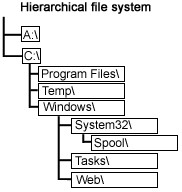
\includegraphics[width=0.27\linewidth]{hierarchy}
	\label{fig:hierarchy}
	\end{figure}
		\begin{enumerate}[(A)]
			\item Preorder depth-first traversal
			\item Postorder depth-first traversal
			\item Inorder depth-first traversal
			\item Breadth-first traversal
		\end{enumerate}
	\end{Q}
    

\question{2}{(3+3+3pts) Tree Structure and Traversal}
	
	Answer the following questions for the tree shown below \textbf{according to  the definition specified in the lecture slides}.
	
	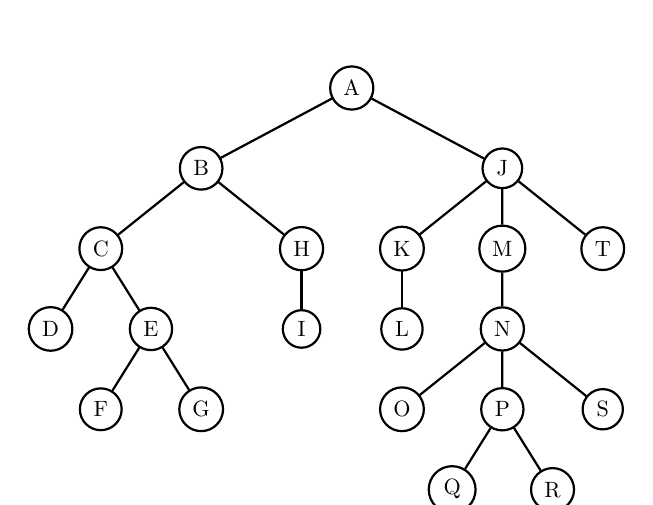
\begin{tikzpicture}
	[thick,scale=0.85, every node/.style={scale=0.8}]

	\node [circle,draw] {A}
	child {node [circle,draw] {B}
		child {node [circle,draw] {C}
			child {node [circle,draw] {D}}
			child {node [circle,draw] {E}
				child {node [circle,draw] {F}}
				child {node [circle,draw] {G}}
			}
		}
		child [missing] {}
		child {node [circle,draw] {H}
			child {node [circle,draw] {I}}
		}
	}	
	child [missing] {}	
	child [missing] {}	
	child {node [circle,draw] {J}
		child {node [circle,draw] {K}
			child {node [circle,draw] {L}}
		}
		child {node [circle,draw] {M}
			child {node [circle,draw] {N}
				child {node [circle,draw] {O}}
				child {node [circle,draw] {P}
					child {node [circle,draw] {Q}}
					child {node [circle,draw] {R}}	
				}
				child {node [circle,draw] {S}}
			}
		}
		child {node [circle,draw] {T}}
	};
	\end{tikzpicture}
	\begin{Q} Please specify: 
	\begin{enumerate}[1.]
		\item The \textbf{children} of the \textbf{root node} with their \textbf{degree} respectively.\\
	  \textup{B, J; deg(B) = 2, deg(J) = 3.}
		\item All \textbf{leaf nodes} in the tree with their \textbf{depth} respectively.\\
		\textup{F, G, Q, R; Depth of F and G are 4, Q and R are 5.}
		\item The \textbf{height} of the tree.\\
		\textup{5.}
		\item The \textbf{ancestors} of O. \\
		\textup{A, J, M, N, O.}
		\item The \textbf{descendants} of C.\\
		\textup{C, D, E, F, G.}
		\item The \textbf{path} from A to S.\\
		\textup{(A, J, M, N, S).}
	\end{enumerate}
	\end{Q}


	For the following two questions, traverse the \textbf{subtree} of the tree shown above with specified root.\\
	
	Note: Form your answer in the following steps.
	\begin{enumerate}[1.]
		\item Decide on an appropriate \textbf{data structure} to implement the traversal.
		\item When you are pushing the children of a node into a \textbf{queue}, please push them alphabetically i.e. from left to right; when you are pushing the children of a node into a \textbf{stack}, please push them in a reverse order i.e. from right to left. 
		\item \textbf{Show all current elements in your data structure at each step} clearly  . \textbf{Popping a node} or \textbf{pushing a sequence of children} can be considered as one single step.
		\item \textbf{Write down your traversal sequence} i.e. the order that you pop elements out of the data structure.
	\end{enumerate}
	
	Please refer to the examples displayed in the lecture slide for detailed implementation of traversal in a tree using the data structure.

	
	\vspace{0.1cm}
	\begin{Q} 
		Run \textbf{Depth First Traversal} in the subtree with root B.
	\end{Q}

	\vspace{0.5cm}
	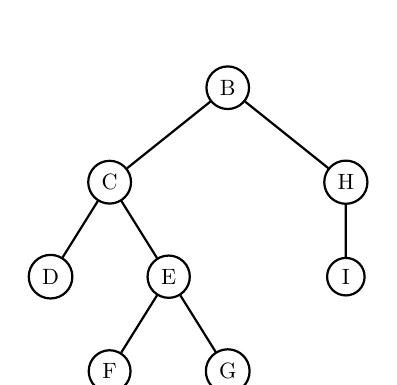
\begin{tikzpicture}
		[thick,scale=1.0, every node/.style={scale=0.8}]
		\node [circle,draw] {B}
		child {node [circle,draw] {C}
				child {node [circle,draw] {D}}
				child {node [circle,draw] {E}
					child {node [circle,draw] {F}}
					child {node [circle,draw] {G}}
				}
		}	
		child [missing] {}
		child {node [circle,draw] {H}
			child {node [circle,draw] {I}}
		};
	\end{tikzpicture}\\
	\textup{We use stack to implement the traversal. Each step, we pop the top elment and then push all its children into the stack.}\\
	\\
	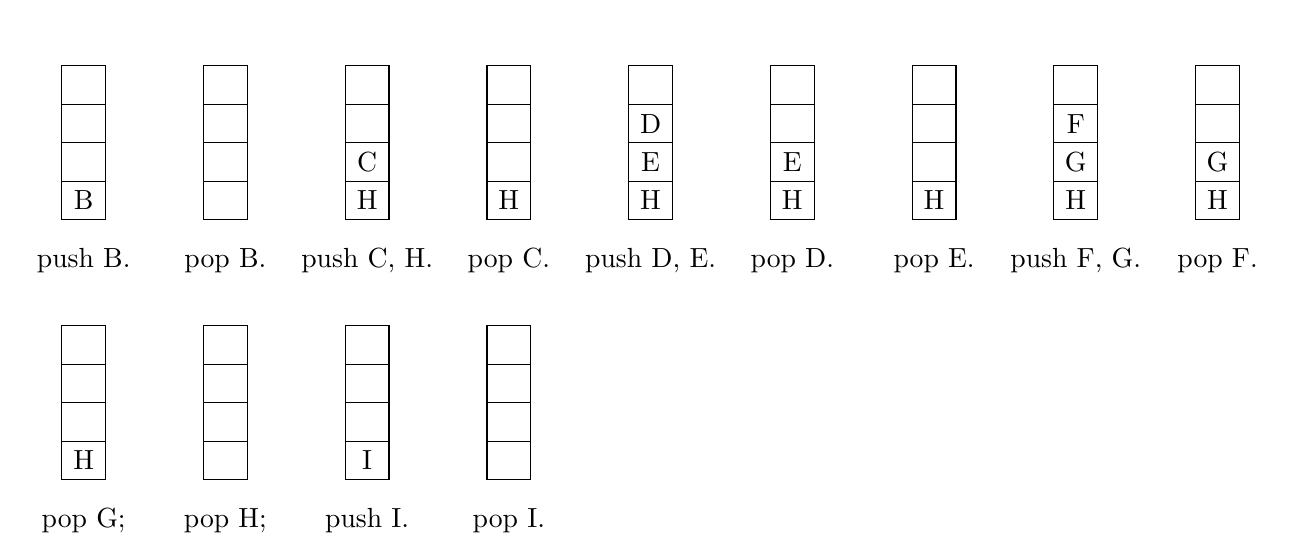
\begin{tikzpicture}[
    stack/.style={rectangle split, rectangle split parts=#1,draw, anchor=center, node distance=1.8cm}, node distance=1.5cm
	]
		\node[stack=4](A){
			\nodepart{one}\textcolor{white}{M}
			\nodepart{two}\textcolor{white}{M}
			\nodepart{three}\textcolor{white}{M}
			\nodepart{four}B
		};
		\node[below of=A] (At){
			push B.
		};

		\node[stack=4, right of=A](B) {
			\nodepart{one}\textcolor{white}{M}
			\nodepart{two}\textcolor{white}{M}
			\nodepart{three}\textcolor{white}{M}
			\nodepart{four}\textcolor{white}{M}
		};
		\node[below of=B] {
			pop B.
		};
		
		\node[stack=4, right of=B](C) {
			\nodepart{one}\textcolor{white}{M}
			\nodepart{two}\textcolor{white}{M}
			\nodepart{three}C
			\nodepart{four}H
		};
		\node[below of=C] {
			push C, H.
		};

		\node[stack=4, right of=C](D) {
			\nodepart{one}\textcolor{white}{M}
			\nodepart{two}\textcolor{white}{M}
			\nodepart{three}\textcolor{white}{M}
			\nodepart{four}H
		};
		\node[below of=D] {
			pop C.
		};

		\node[stack=4, right of=D](E) {
			\nodepart{one}\textcolor{white}{M}
			\nodepart{two}D
			\nodepart{three}E
			\nodepart{four}H
		};
		\node[below of=E] {
			push D, E.
		};

		\node[stack=4, right of=E](F) {
			\nodepart{one}\textcolor{white}{M}
			\nodepart{two}\textcolor{white}{M}
			\nodepart{three}E
			\nodepart{four}H
		};
		\node[below of=F] {
			pop D.
		};

		\node[stack=4, right of=F](G) {
			\nodepart{one}\textcolor{white}{M}
			\nodepart{two}\textcolor{white}{M}
			\nodepart{three}\textcolor{white}{M}
			\nodepart{four}H
		};
		\node[below of=G] {
			pop E.
		};

		\node[stack=4, right of=G](I) {
			\nodepart{one}\textcolor{white}{M}
			\nodepart{two}F
			\nodepart{three}G
			\nodepart{four}H
		};
		\node[below of=I] {
			push F, G.
		};

		\node[stack=4, right of=I](J) {
			\nodepart{one}\textcolor{white}{M}
			\nodepart{two}\textcolor{white}{M}
			\nodepart{three}G
			\nodepart{four}H
		};
		\node[below of=J] {
			pop F.
		};\\

		\node[stack=4, below of=At](K) {
			\nodepart{one}\textcolor{white}{M}
			\nodepart{two}\textcolor{white}{M}
			\nodepart{three}\textcolor{white}{M}
			\nodepart{four}H
		};
		\node[below of=K] {
			pop G;
		};
		
		\node[stack=4, right of=K](L) {
			\nodepart{one}\textcolor{white}{M}
			\nodepart{two}\textcolor{white}{M}
			\nodepart{three}\textcolor{white}{M}
			\nodepart{four}\textcolor{white}{M}
		};
		\node[below of=L] {
			pop H;
		};

		\node[stack=4, right of=L](M) {
			\nodepart{one}\textcolor{white}{M}
			\nodepart{two}\textcolor{white}{M}
			\nodepart{three}\textcolor{white}{M}
			\nodepart{four}I
		};
		\node[below of=M] {
			push I.
		};

		\node[stack=4, right of=M](N) {
			\nodepart{one}\textcolor{white}{M}
			\nodepart{two}\textcolor{white}{M}
			\nodepart{three}\textcolor{white}{M}
			\nodepart{four}\textcolor{white}{M}
		};
		\node[below of=N] {
			pop I.
		};
		
	\end{tikzpicture}\\
	\textup{Pop sequence: B, C, D, E, F, G, H, I.}\\

	\begin{Q} 
		Run \textbf{Breadth First Traversal} in the subtree with root N.
	\end{Q}

	\vspace{0.5cm}
	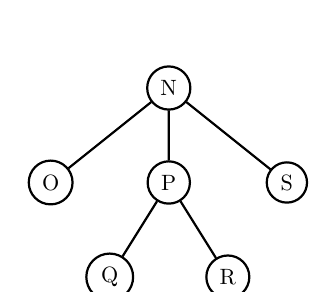
\begin{tikzpicture}
		[thick,scale=1, every node/.style={scale=0.8}]
		\node [circle,draw] {N}
			child {node [circle,draw] {O}}
			child {node [circle,draw] {P}
				child {node [circle,draw] {Q}}
				child {node [circle,draw] {R}}	
			}
			child {node [circle,draw] {S}};
	\end{tikzpicture}\\
We use queue to implement traversal.\\
\\
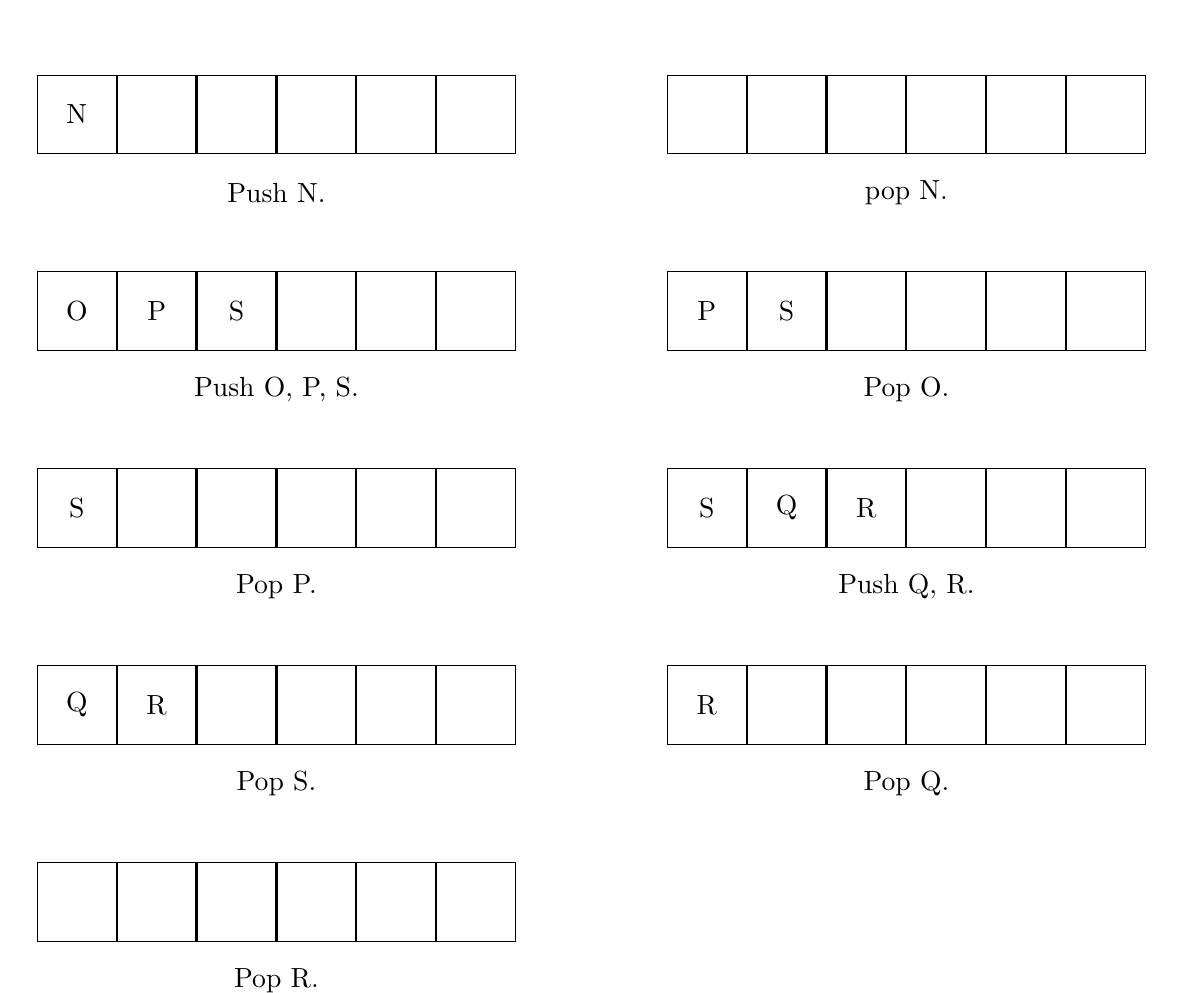
\begin{tikzpicture} [array/.style={matrix of nodes, nodes={draw, minimum size = 10mm, anchor=center}, nodes in empty cells, node distance=8cm}]
	\matrix(m1) 
	[array]
	{
		N& & & & &\\
	};
	\node[below of=m1]{
		Push N.
	};

	\matrix(m2) 
	[array, right of=m1]
	{
		& & & & &\\
	};
	\node[below of=m2]{
		pop N.
	};

	\matrix(m3) 
	[array, below of=m1,node distance=2.5cm]
	{
		O & P & S & & &\\
	};
	\node[below of=m3]{
		Push O, P, S.
	};

	\matrix(m4) 
	[array, right of=m3]
	{
		P & S &  & & &\\
	};
	\node[below of=m4]{
		Pop O.
	};

	\matrix(m5) 
	[array, below of=m3,node distance=2.5cm]
	{
		S &  &  & & &\\
	};
	\node[below of=m5]{
		Pop P.
	};

	\matrix(m6) 
	[array, right of=m5]
	{
		S & Q & R & & &\\
	};
	\node[below of=m6]{
		Push Q, R.
	};

	\matrix(m7) 
	[array, below of=m5,node distance=2.5cm]
	{
		Q & R &  & & &\\
	};
	\node[below of=m7]{
		Pop S.
	};

	\matrix(m8) 
	[array, right of=m7]
	{
		R &  &  & & &\\
	};
	\node[below of=m8]{
		Pop Q.
	};

	\matrix(m9) 
	[array, below of=m7,node distance=2.5cm]
	{
		 &  &  & & &\\
	};
	\node[below of=m9]{
		Pop R.
	};
\end{tikzpicture}\\
\\
Pop sequence: N, O, P, S, Q, R.


\newpage


\question{3}{(2+3pts) Recurrence Relations}
	For each question, find the asymptotic order of growth of $T(n)$ i.e. find a function $g$ such that $T(n) = O(g(n))$. You may ignore any issue arising from whether a number is an integer. You can make use of the Master Theorem, Recursion Tree or other reasonable approaches to solve the following recurrence relations.

	\textit{Note: \textbf{Mark or circle} your final answer clearly.\\ }

	\begin{Q} $T(n) = 4T(n/2) + 42\sqrt{n}$.
	\end{Q}
	$$
	a = 4, b= 2, \log_b a = \log_2 4 = 2.\\
	$$
	Since $2 < \frac12$, by Master Theorem, $T(n) = O(n^2)$.\\

	\begin{Q} $T(n) = T(\sqrt{n}) + 1$. You may assume that $T(2)=T(1)=1$.
	\end{Q}
	We assume that $T(n) = O(\log(\log n))$.\\
	For any $m = \sqrt n$, we have $T(\sqrt n) \le \log(\log\sqrt n)$.\\
	Therefore
	\begin{align*}
		T(n) &= T(\sqrt n) + 1\\
		&\le \log(\log\sqrt n) + 1\\
		& = \log(\log \sqrt n) + \log 2\\
		& = \log(2\log n^{\frac12})\\
		&= \log(\log n)
	\end{align*}
By using methematical induction, we know that $T(n) = O(\log(\log n))$


\newpage
\question{3}{(7+6+6pts) Divide and Conquer Algorithm}

\begin{Q}
In this problem, we will find an alternative approach to the merge step in Merge Sort named \textbf{Slice Merge} . Suppose $A$ and $B$ are sorted arrays with possibly different lengths, and let $n=len(A)+len(B)$. You may assume $n$ is a power of two and all $n$ elements have distinct value. The slice merge algorithm, \textbf{smerge(A,B)}, merges $A$ and $B$ into a single sorted arrays as follows:

\begin{figure}[htbp]
	\centering
	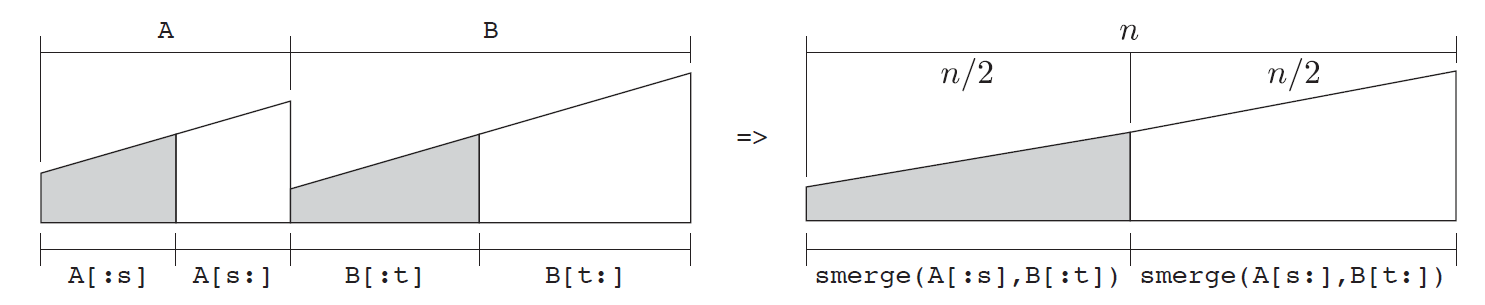
\includegraphics[width=1.0\linewidth]{2}
\end{figure}

\textbf{Step 1:} Find index $s$ for subarray A and index $t$ for subarray B ($s+t=\dfrac{n}{2}$) to form two prefix subarrays \texttt{A[:s]} and \texttt{B[:t]}, such that \texttt{A[:s]} $\cup$ \texttt{B[:t]} contains the smallest $\dfrac{n}{2}$ elements in all $n$ elements of $A\cup B$.\\
 
\textbf{Step 2:} Recur for \texttt{X = smerge(A[:s], B[:t])} and \texttt{Y = smerge(A[s:], B[t:])} respectively to reorder and merge them. Return their concatenation $X+Y$, a sorted array containing all elements in $A\cup B$.\\
 
 For example, if $A=[1, 3, 4, 6, 8]$ and $B=[2, 5, 7]$, we should find $s=3$ and $t=1$ and then recursively compute:
 
\centerline{\texttt{smerge([1, 3, 4], [2]) + smerge([6, 8], [5, 7]) = [1, 2, 3, 4] + [5, 6, 7, 8]}}

\vspace{0.5cm}
\begin{enumerate}[1.]
\item  Describe an algorithm for Step 1 to find indices $s$ and $t$ in $O(n)$ time using $O(1)$ additional space. Write down your main idea briefly (or pseudocode if you would like to) and analyse the runtime complexity of your algorithm below. You may assume array starts at index 1. \textbf{(2pts)}\\
\begin{algorithm}[H]
	\caption{Step 1 of Slice Merge}
	\begin{algorithmic}[1]
		\Function {findSandT}{A, B}
			\State $half \gets \lfloor(A.lenth + B.length) / 2 \rfloor$
			\State $s \gets 0$
			\State $t \gets 0$
			\For{$j \gets 1 $ \textbf{to} $half$}
				\If{$A[s + 1] < B[t + 1]$}
					\State $s \gets s + 1$
				\Else
					\State $t \gets t + 1$
				\EndIf
			\EndFor
		\State \Return s, t
		\EndFunction
	\end{algorithmic}
\end{algorithm}
\textup{Since} $A.length + B.length = n$\textup{, the runtime complexity should be} $O(2 \cdot\frac12 n) = O(n)$


\item Write down a recurrence for the runtime complexity of \texttt{smerge(A,B)} when $A \cup B$ contains a total of $n$ items. Solve it using the Master Theorem and show your calculation below.\textbf{(2pts)}\\
Note: Write your answer for time complexity in asymptotic order form i.e. $T(n)=O(g(n))$.\\
\\
$T(n) = 2T(\frac n 2) + cn $\\
$$
 a = 2, b = 2, \log_b a = 1 = d
$$
\textup{By Master Theorem, }$T(n) = O(n\log n)$

\item Recall the merge step \texttt{merge(A,B)} to combine two subarrays of length $n/2$ in the Merge Sort algorithm covered in our lecture slides. Compare the runtime complexity of \texttt{smerge(A,B)} with \texttt{merge(A,B)}.\textbf{(1pts)}\\
\\
\textup{The runtime complexity of }$merge(A, B)$\textup{ is }$O(n)$\textup{, while the runtime complexity of }$smerge(A, B)$\textup{ is }$O(n \log n)$. \textup{Therefore }$T_{smerge}(n) > T_{merge}(n)$.\\
\item  Replace \texttt{merge(A,B)} by \texttt{smerge(A,B)} in the merge stage of Merge Sort to develop a new sorting method namely \textbf{S-Merge Sort}. Write down a recurrence for the runtime complexity of S-Merge Sort. Solve it and show your calculation below.\textbf{(2pts)}\\
Note: Write your answer for time complexity in asymptotic order form i.e. $T(n)=O(g(n))$.\\
\\
\begin{align*}
	T(n) &= 2 T(n / 2) + n\log n\\
	a &= 2, b = 2,\\ c^{crit} &= \log_a b = 1	= d.
\end{align*}
\textup{Since }$f(n) = n\log n = n^{c^{crit}}\log n$\textup{, by Master Theorem,}
$$
T(n) =O\left( n\log^2n\right)
$$




\end{enumerate}
\end{Q}
\newpage

\begin{Q}
	There are $n$ students in SIST and each student $i$ has $2$ scores $A_i$ and $P_i$, score in Algorithms and Data Structures course and score in Probabilty and Statistics course respectively. Students $i$, $j$ could form a mutual-help pair in CS101 class if and only
	if $A_i < A_j$ and $P_i > P_j$ . How many possible mutual-help pairs $(i,j)$ could be formed in CS101 class? 
	
	Design an efficient algorithm  to figure out this problem. For comparison, our
	algorithm runs in $O(n \log n)$ time. (Hint: how to count inversions?)\\

	Note: Your answer should be consistent with the template we provide in Problem 0 Example.
\end{Q}

First, sort the students according to A in ascending order using mergesort, which has been showed in the class. After that, sort the students again according to P in descending order. Meanwhile, count the inversions of P using merge sort. The inversions of P should be the answer. The complete algorithm is described as follows.\\
\begin{algorithm}[H]
	\caption{Question 10 CountInversionsByMergesort}
	\begin{algorithmic}[1]
		\Function{CountInversionsByMergesort}{StudentArr, left, right, mid}
		\State $count \gets 0$
		\State $length \gets right - left + 1$
		\State $tempArr \gets$ an array of the type of the elements in $StudentArr$ with length of $length$
		\State $leftSubLength \gets mid - left$
		\State $rightSubLength \gets right - mid + 1$
		\State $leftptr \gets 0$
		\State $rightptr \gets 0$
		\State $tempptr \gets 0$
		\While{$leftptr < leftSubLength $ and $rightptr < rightSubLength$}
			\If{$StudentArr[left + leftptr].P > StudentArr[mid + rightptr].P$}
				\State $tempArr[tempptr] \gets StudentArr[left + leftptr]$
				\State $leftptr \gets leftptr + 1$
				\State $count \gets count + rightSubLength - rightptr - 1$
			\Else
				\State $tempArr[tempptr] \gets StudentArr[mid + rightptr]$
				\State $rightptr \gets rightptr + 1$
			\EndIf
			\State $tempptr \gets tempptr + 1$
		\EndWhile
		\While{$leftptr < leftSubLength$}
			\State $tempArr[tempptr] \gets StudentArr[left + leftptr]$
			\State $leftptr \gets leftptr + 1$
			\State $tempptr \gets tempptr + 1$
		\EndWhile
		\While{$rightptr < rightSubLength$}
			\State $tempArr[tempptr] \gets StudentArr[mid + rightptr]$
			\State $rightptr \gets rightptr + 1$
			\State $tempptr \gets tempptr + 1$
		\EndWhile
		\algstore{myalg}
	\end{algorithmic}	
\end{algorithm}

\begin{algorithm} [H]
	\begin{algorithmic}[1]
		\algrestore{myalg}
		\For{$i \gets 1$ \textbf{to} $length$}
			\State $StudentArr[left + i - 1] \gets tempArr[i]$
		\EndFor
		\State \Return count
		\EndFunction
	\end{algorithmic}	
\end{algorithm}

\begin{algorithm} [H]
	\caption{Question 10 CountPairs}
	\begin{algorithmic}[1]
		\Function{CountPairs}{StudentArr, left, right}
		\If{left >= right} 
			\State return 0
		\EndIf
		\State $mid \gets \lfloor (right - left )/ 2 \rfloor+ left$
		\State $countleft \gets CountPairs(StudentArr, left, mid)$
		\State $countright \gets CountPairs(StudentArr, mid + 1, right)$
		\State $count \gets countleft + countright + CountInversionsByMergesort(StudentArr, left, right, mid)$
		\State \Return $count$
		\EndFunction
	\end{algorithmic}
\end{algorithm}

\begin{algorithm} [H]
	\caption{Quetion 10 Complete Algorithm}
	\begin{algorithmic} [1]
		\Function{Main}{StudentArr}
		\State sort $StudentArr$ according to $A$ of each element in ascending order use $Mergesort$.
		\State $answer \gets CountPairs(StudentArr, 1, StudentArr.length)$
		\State \Return answer
		\EndFunction
	\end{algorithmic}
\end{algorithm}

\begin{align*}
	T(n)_{CountPairs} &= 2T(n/2)_{CountPairs} + n \\
\end{align*}
By master Theorem, 
\begin{align*}
	a & = 2\\
	b & = 2\\
	\log_b a & = 1 = d\\
	T(n)_{CountPairs}& = O(n\log n)\\
\end{align*}
Therefore, 
\begin{align*}
	T(n)_{Main} &= T(n)_{CountPairs} + T(n)_{Mergesort} \\
							&= O(2n\log n) = O(n\log n)
\end{align*}
\newpage

\begin{Q}
Suppose you are a teaching assistant for CS101, Fall 2077. The TA group has a collection of $n$ suspected code solutions from $n$ students for the programming assignment, suspecting them of academic plagiarism. It is easy to judge whether two code solutions are equivalent with the help of ``plagiarism detection machine'', which takes two code solutions \texttt{(A,B)} as input and outputs \texttt{isEquivalent(A, B)} $\in$ \{\texttt{True}, \texttt{False}\} i.e. whether they are equivalent to each other.

TAs are curious about whether there exists a \textbf{majority} i.e. an \textbf{equivalent class of size $>\dfrac{n}{2}$} among all subsets of the code solution collection. That means, in such a subset containing more than $\dfrac{n}{2}$ code solutions, any two of them are equivalent to each other.

Assume that the only operation you can do with these solutions is to pick two of them and plug them into the plagiarism detection machine. Please show TAs' problem can be sloved using $O(n\log n)$ invocations of the plagiarism detection machine.\\

Note: Your answer should be consistent with the template we provide in Problem 0 Example.

\noindent
\end{Q}
Find majority recursively, if the array has majority, record the element.
Each step, seperate the array into two subarray, each contains $\frac n 2$ elements.\\
Check whether two subarrays contains majority recursively. If both subarray has majority then the majority of the current array should be the majority of the subarray. If one of subarray has majority or they have different majority, then count the majority in another subarray to see if this element is the majority of the current array. This can be finished in $O(n)$. If neither of the array has majority, then the current array won't have majority.\\
If there's only one elment in the array, the majority should be that element.\\
The complete algorithm is described as follows.\\
\begin{algorithm}[H]
	\caption{Q11 CountElement}
	\begin{algorithmic}[1]
		\Function{CountElement}{StudentSolution, element, left, right}
			\State $count \gets 0$
			\For{$i \gets left$ \textbf{to} $right$}
				\If{$isEquivalent(element, StudentSolution[i])$}
					\State $count \gets count + 1$
				\EndIf
			\EndFor
		\EndFunction
	\end{algorithmic}
\end{algorithm}

\begin{algorithm}[H]
	\caption{Q11 CountMajority}
	\begin{algorithmic}[1]
		\Function{CountMajority}{StudentSolution, left, right}
			\If{ $left == right$}
				\State $hasMajority \gets $ \textbf{true}
				\State $major \gets StudentSolution[left]$
				\State \Return hasMajority, major
			\EndIf
			\algstore{mystore}
		\end{algorithmic}
	\end{algorithm}
	\begin{algorithm}[H]
		\begin{algorithmic}[1]
			\algrestore{mystore}
			\State $mid \gets \lfloor (right - left) / 2\rfloor + left$
			\State $length \gets right - left + 1$
			\State $hasMajorityLeft,\,majorLeft \gets CountMajority(StudentSolution, left, mid)$
			\State $hasMajorityRight,\,majorRight \gets CountMajority(StudentSolution, mid + 1, right)$
			\If{$hasMajorityLeft $ \textbf{and} $hasMajorityRight$ \textbf{and} $isEquivalent(majorLeft, majorRight)$}
				\State $hasMajority \gets $ \textbf{true}
				\State $major \gets majorLeft$
			\ElsIf{$hasMajorityLeft$ \textbf{and} $CountElement(StudentSolution, majorLeft, left, right) > \lfloor \frac {length} {2}\rfloor$ }
				\State $hasMajority \gets $ \textbf{true}
				\State $major \gets majorLeft$
			\ElsIf{$hasMajorityRight$ \textbf{and} $CountElement(StudentSolution, majorRight, left, right) > \lfloor \frac {length} {2}\rfloor$}
				\State $hasMajority \gets $ \textbf{true}
				\State $major \gets majorRight$
			\Else
				\State $hasMajority \gets $ \textbf{false}
				\State $major \gets$ \textbf{null}
			\EndIf
			\State \Return hasMajority, major
		\EndFunction
	\end{algorithmic}
\end{algorithm}


\begin{algorithm}[H]
	\caption{Q11 Complete Algorithm}
	\begin{algorithmic}[1]
		\Function{Main}{StudentSolution}
			\State $hasMajority, major \gets CountMajority(StudentSolution, 1, StudentSolution.length)$
			\State \Return $hasMajority$
		\EndFunction
	\end{algorithmic}
\end{algorithm}

The time complexity of $CountElement$ is $O(n)$. The time complexity of $CountMajority$ can be written as $T(n) = 2T(n / 2) + O(n)$. By Master Theorem, 
\begin{align*}
	a &= 2\\
	b &= 2\\
	\log_b a &= 1 = d \\
T(n) &= O(n \log n)
\end{align*}


\end{document}